\documentclass{article}
\usepackage[final]{nips_2017}

% to compile a camera-ready version, add the [final] option, e.g.:
% \usepackage[final]{nips_2017}

\usepackage[utf8]{inputenc} % allow utf-8 input
\usepackage[T1]{fontenc}    % use 8-bit T1 fonts
\usepackage{hyperref}       % hyperlinks
\usepackage{url}            % simple URL typesetting
\usepackage{booktabs}       % professional-quality tables
\usepackage{amsfonts}       % blackboard math symbols
\usepackage{nicefrac}       % compact symbols for 1/2, etc.
\usepackage{microtype}      % microtypograph

\usepackage{graphicx}
\usepackage{amsmath}

\bibliographystyle{plain}

\title{Reproduction: Unsupervised Monocular Depth Estimation with Left-Right Consistency}

% The \author macro works with any number of authors. There are two
% commands used to separate the names and addresses of multiple
% authors: \And and \AND.
%
% Using \And between authors leaves it to LaTeX to determine where to
% break the lines. Using \AND forces a line break at that point. So,
% if LaTeX puts 3 of 4 authors names on the first line, and the last
% on the second line, try using \AND instead of \And before the third
% author name.

\author{
	Andrija Djurisic\\
	Faculty of Mathematics, Belgrade\\
	\texttt{andrija.m.djurisic@gmail.com} \\
	%% examples of more authors
	%% \And
	%% Coauthor \\
	%% Affiliation \\
	%% Address \\
	%% \texttt{email} \\
	%% \AND
	%% Coauthor \\
	%% Affiliation \\
	%% Address \\
	%% \texttt{email} \\
	%% \And
	%% Coauthor \\
	%% Affiliation \\
	%% Address \\
	%% \texttt{email} \\
	%% \And
	%% Coauthor \\
	%% Affiliation \\
	%% Address \\
	%% \texttt{email} \\
}

\begin{document}
	% \nipsfinalcopy is no longer used
	
	\maketitle
	
%	\begin{abstract}
%		The abstract paragraph should be indented \nicefrac{1}{2}~inch
%		(3~picas) on both the left- and right-hand margins. Use 10~point
%		type, with a vertical spacing (leading) of 11~points.  The word
%		\textbf{Abstract} must be centered, bold, and in point size 12. Two
%		line spaces precede the abstract. The abstract must be limited to
%		one paragraph.
%	\end{abstract}
	
\section{Introduction}
In this paper Godard et. al. \cite{DBLP:journals/corr/GodardAB16} are presenting unsupervised method for solving depth estimation problem. 

% Most existing approaches treat depth estimation as a supervised regression problem and as a result, require vast quantities of corresponding ground truth depth data for training.
Most learning based methods for monocular depth estimation rely on the availability of ground truth depth data aligned with each input image. These methods take color-depth pairs as an input during the training and learn to directly predict depth maps from color images. One such method is \emph{DispNet} \cite{DBLP:journals/corr/MayerIHFCDB15} which introduced fully convolutional architecture similar to one used in this paper. 

Capturing reliable depth data is both expensive and time-consuming and as an alternative stereo data is much easier to capture requiring only two synchronized cameras. Authors are proposing novel method which takes color image captured from the left camera as an input and color image captured from the right camera as a target during the training. Their convolutional neural network then learns to generate per pixel disparities that produce the right target image by shifting pixels from the left input image using differentiable image sampler \cite{DBLP:journals/corr/GodardAB16}.

% Depth can be then trivially recovered from the predicted disparity.
% Depth tells us how much each pixel moves between the images in a stereo pair.
\section{Method}
At training time, we have access to two images $I^l$ and $I^r$, corresponding to the left and right color images from a calibrated stereo pair, captured at the same moment in time. The idea is to find the disparity $d^r$ that, when applied to the left image, it would enable us to reconstruct the right image. We will refer to the reconstructed image $I^l(d^r)$ as $\tilde{I^r}$. Similarly, we can also estimate the left image given the right one, $\tilde{I^l} = I^r(d^l)$. Assuming that the images are rectified \cite{Hartley:2003:MVG:861369}, for a given disparity $d$, the baseline distance between the cameras $b$ and the camera focal length $f$, we can calculate the depth $\hat{d}=bf/d$.

% Authors showed results using two types of encoders - VGG \cite{DBLP:journals/corr/SimonyanZ14a} and Resnet50 \cite{DBLP:journals/corr/HeZRS15}.
Network consists of encoder and decoder part. The encoder part contains only convolutional layers with occasional strides of $2$, resulting in a total downsampling factor of $128$. Decoder part of the network gradually and nonlinearly upsamples the feature maps, taking into account the features from the encoder part. This is done by a series of up-convolutional and convolutional layers. Network output disparity predictions at four different scales (\emph{disp4} to \emph{disp1})\footnote{https://github.com/andrijazz/playground/tree/master/docs/imgs/arch.png}.

The training loss is split into three portions:
\begin{itemize}
	\item $C_{ap}$ - Appearance matching loss encourages the reconstructed input to be similar to the corresponding training input and it is defined as a combination of an $L1$ and single scale SSIM loss:
	\begin{align*}
		C_{ap}^l &= \frac{1}{N}\sum_{i,j}\alpha \frac{1 - SSIM(I_{ij}^l, \tilde{I}_{ij}^l)}{2} + (1 - \alpha)  \left\lVert I_{ij}^l - \tilde{I}_{ij}^l \right\rVert
	\end{align*}
	
	\item $C_{ds}$ - Disparity smoothness loss encourages smooth disparities:
	\begin{align*}
		C_{ds}^l &= \frac{1}{N}\sum_{i,j}|\partial_x d_{ij}^l|e^{-|| \partial_x I_{ij}^l ||} + |\partial_y d_{ij}^l|e^{-|| \partial_y I_{ij}^l ||}
	\end{align*}
	
	\item $C_{lr}$ - Makes left and right disparities consistent with each other. It is defined as $L1$ penalty: 
	\begin{align*}
		C_{lr}^l &= \frac{1}{N}\sum_{i,j}|d_{ij}^l - d_{ij + d_{ij}^l}^r|
	\end{align*}	
\end{itemize}

Loss is calculated at each scale $s$ in order to handle different resolutions. The resulting loss function at each scale is:
\begin{align*}
	C_s &= \alpha_{ap}(C_{ap}^{l} + C_{ap}^{r}) + \alpha_{ds}(C_{ds}^{l} + C_{ds}^{r}) +
\alpha_{lr}(C_{lr}^{l} + C_{lr}^{r})
\end{align*}

forming the total loss as the sum  $C = \sum_{s=1}^{4}\lambda_sC_s$.


\section{Implementation}
   
I implemented the model in TensorFlow \cite{DBLP:journals/corr/AbadiABBCCCDDDG16}. Please take a look at my code\footnote{https://github.com/andrijazz/playground/tree/master/monodepth} for more details. Model was trained on Tesla K80 GPU and it took about 48 hours to complete. I used identical subset of KITTI \cite{Menze2018JPRS} dataset that authors used for their experiments which consists of $30000$ images. It was trained for $50$ epochs in batches of $2$. Weighting of losses was set in the following manner: $\alpha_{ap} = 1$, $\alpha_{ds} = 0.1$, $\alpha_{lr} = 1$. Learning rate was set to $\lambda = 10^{-4}$ and kept constant for the first $30$ epochs. After that it is divided by $2$ every $10$ epochs until the end \cite{DBLP:journals/corr/GodardAB16}. Results are presented in the following section\footnote{For more detailed results please take a look at github readme file.}.

To improve performance I am planning to implement data augmentation and rework data loading pipeline by exploiting \textbf{tf.data}\footnote{https://www.tensorflow.org/api\_docs/python/tf/data} library of TensorFlow, as well as to train the model with more data (on Cityscapes dataset\cite{DBLP:journals/corr/CordtsORREBFRS16}). I am expecting that this will improve training time as well as quality of produced images. The best results presented in the paper were achieved by feeding concatenation of both left and right views as an input into the network so I will definately try out that as well.

% future work
% Resnet 50
% Post-processing
% your own observations about the paper, e.g. analysis of robustness, was the paper difficult to reproduce given the details in the paper; most important tricks in implementation etc. 

\section{Results}
\begin{figure}[h]
	\centering
	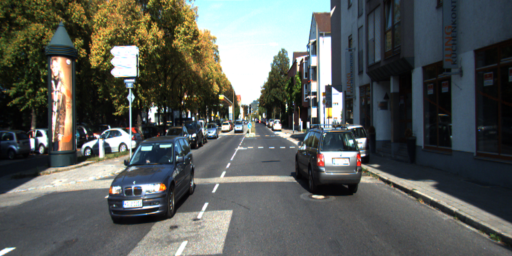
\includegraphics[width=180px]{imgs/8_left.png}
	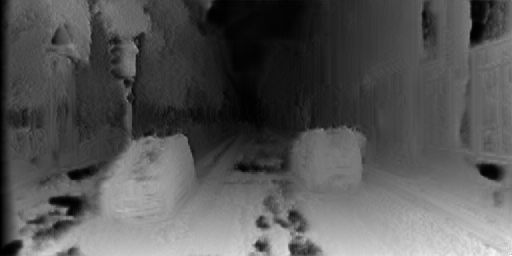
\includegraphics[width=180px]{imgs/8_disp.png}\\
	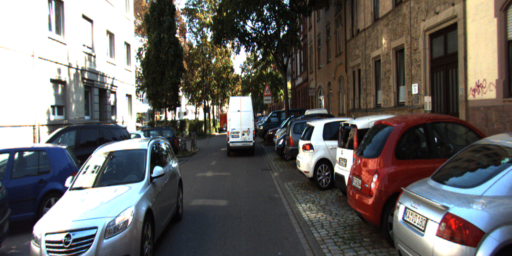
\includegraphics[width=180px]{imgs/32_left.png}
	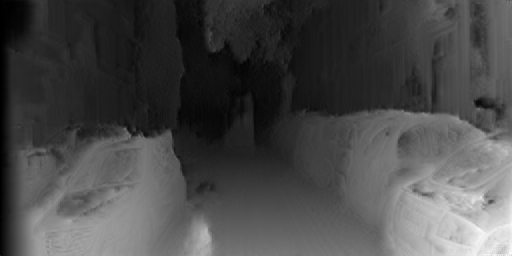
\includegraphics[width=180px]{imgs/32_disp.png}\\
%	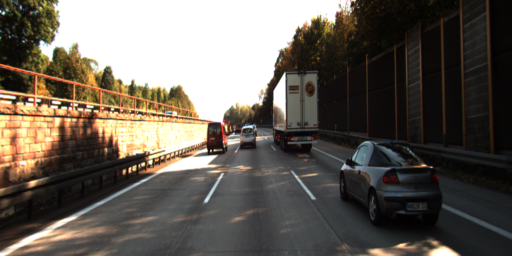
\includegraphics[width=140px]{imgs/46_left.png}
%	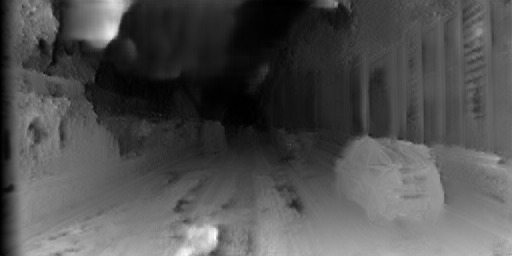
\includegraphics[width=140px]{imgs/46_disp.png}	
	\caption{Images on the left are input to the model and images on right are produced disparities.}
\end{figure}

%\begin{table}[t]
%	\caption{Results}
%	\label{results}
%	\centering
%	\begin{tabular}{ll}
%		\toprule
%		Metric     	& Result \\
%		\midrule
%		Abs Rel 	& 0.2860  \\
%		Sq Rel     	& 33.3344 \\
%		RMSE     	& 325.825 \\
%		RMSE log	& 0.623	  \\
%		\bottomrule
%	\end{tabular}
%\end{table}

%   abs_rel,     sq_rel,        rms,    log_rms,     d1_all,         a1,        a2,         a3
%	 0.2860,    33.3344,    325.825,      0.623,     50.031,      0.655,      0.772,      0.833


\bibliography{ref}

\end{document}